\documentclass{standalone}
\usepackage{pgfplots}
\usetikzlibrary{decorations.pathmorphing,patterns}
\begin{document}
\begin{tikzpicture}[xscale=0.25,yscale=1]
 	\draw[<->] (-21, 0) -- (21, 0);
  	\draw[->] (0, -2) -- (0, 2);
    %\draw[very thin,color=gray] (-0.1,-1.1) grid (3.9,3.9);
	%\draw[color=blue]   plot (\x,{sin(\x r)}) ; 
	\draw[domain=-20:20,samples=200,blue] plot(\x,{sin(\x r)});
	\draw (18, -1.5) node {$t=\dfrac{5 \, \pi}{\omega_{0}}$};
\end{tikzpicture}
\end{document}